\chapter{Evaluation}

\begin{figure}[h!]
\centering
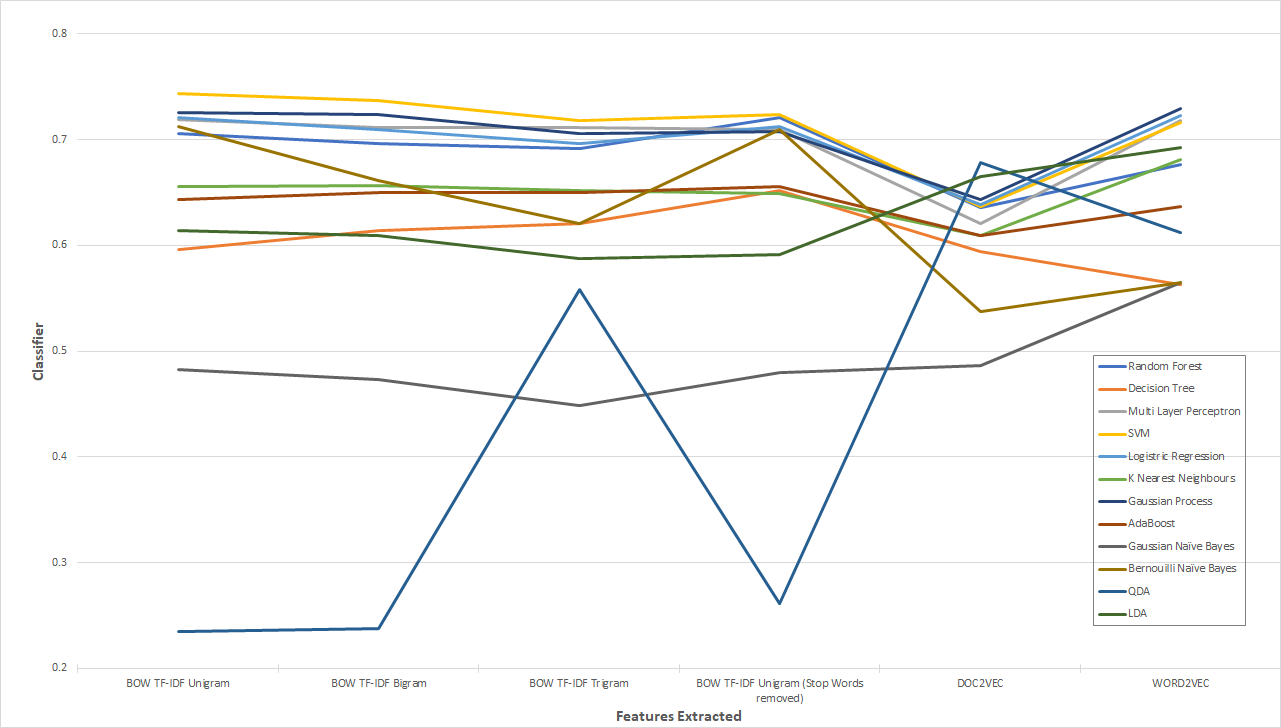
\includegraphics[width=1\textwidth]{evaluation/accuracy_graph.png}
\caption{\label{fig:accuracy} Accuracy Graph}
\end{figure}

\begin{figure}[h!]
\centering
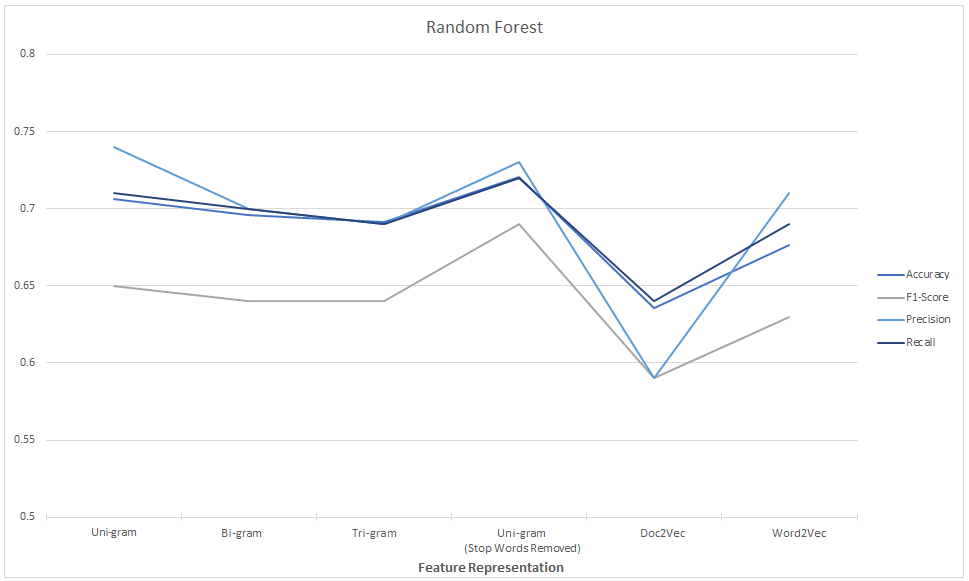
\includegraphics[width=1\textwidth]{evaluation/random_forest_graph.png}
\caption{\label{graph:randomforest} Random Forest Graph}
\end{figure}

% *** ACCURACY ***
\begin{table}[]
\setlength\extrarowheight{5pt}
\begin{tabular}{ccccccc}
\specialrule{1.5pt}{1pt}{1pt}
 & \textbf{Uni-gram} & \textbf{Bi-gram} & \textbf{Tri-gram} & \textbf{\begin{tabular}[c]{@{}c@{}}Uni-gram \\ (No Stop Words)\end{tabular}} & \textbf{Doc2Vec} & \textbf{Word2Vec} \\ \specialrule{1.5pt}{1pt}{1pt}
\textbf{RF} & 0.706 & 0.696 & 0.691 & 0.721 & 0.635 & 0.677 \\ \hline
\rowcolor[HTML]{EFEFEF} 
\textbf{DT} & 0.596 & 0.614 & 0.621 & 0.652 & 0.594 & 0.563 \\ \hline
\textbf{MLP} & 0.719 & 0.711 & 0.711 & 0.709 & 0.621 & 0.718 \\ \hline
\rowcolor[HTML]{EFEFEF} 
\textbf{SVM} & 0.744 & 0.737 & 0.718 & 0.724 & 0.637 & 0.716 \\ \hline
\textbf{LR} & 0.721 & 0.709 & 0.696 & 0.713 & 0.639 & 0.722 \\ \hline
\rowcolor[HTML]{EFEFEF} 
\textbf{KNN} & 0.655 & 0.657 & 0.652 & 0.649 & 0.609 & 0.681 \\ \hline
\textbf{GP} & 0.726 & 0.724 & 0.706 & 0.708 & 0.644 & 0.729 \\ \hline
\rowcolor[HTML]{EFEFEF} 
\textbf{AB} & 0.644 & 0.650 & 0.650 & 0.655 & 0.609 & 0.637 \\ \hline
\textbf{GNB} & 0.483 & 0.473 & 0.448 & 0.479 & 0.486 & 0.565 \\ \hline
\rowcolor[HTML]{EFEFEF} 
\textbf{BNB} & 0.713 & 0.662 & 0.621 & 0.709 & 0.537 & 0.565 \\ \hline
\textbf{QDA} & 0.235 & 0.238 & 0.558 & 0.261 & 0.678 & 0.612 \\ \hline
\rowcolor[HTML]{EFEFEF} 
\textbf{LDA} & 0.614 & 0.609 & 0.588 & 0.591 & 0.665 & 0.693 \\ \hline
\end{tabular}
\caption{Accuracy of Classifiers for different Feature Representations}
\label{Table:accuracy}
\end{table}

% *** F1 SCORE ***
\begin{table}[]
\setlength\extrarowheight{5pt}
\begin{tabular}{ccccccc}
\specialrule{1.5pt}{1pt}{1pt}
 & \textbf{Uni-gram} & \textbf{Bi-gram} & \textbf{Tri-gram} & \textbf{\begin{tabular}[c]{@{}c@{}}Uni-gram \\ (No Stop Words)\end{tabular}} & \textbf{Doc2Vec} & \textbf{Word2Vec} \\ \specialrule{1.5pt}{1pt}{1pt}
\textbf{RF} & 0.65 & 0.64 & 0.64 & 0.69 & 0.59 & 0.63 \\ \hline
\rowcolor[HTML]{EFEFEF} 
\textbf{DT} & 0.59 & 0.58 & 0.6 & 0.63 & 0.56 & 0.54 \\ \hline
\textbf{MLP} & 0.7 & 0.69 & 0.69 & 0.69 & 0.57 & 0.71 \\ \hline
\rowcolor[HTML]{EFEFEF} 
\textbf{SVM} & 0.73 & 0.73 & 0.71 & 0.71 & 0.63 & 0.71 \\ \hline
\textbf{LR} & 0.7 & 0.69 & 0.68 & 0.69 & 0.6 & 0.71 \\ \hline
\rowcolor[HTML]{EFEFEF} 
\textbf{KNN} & 0.62 & 0.62 & 0.62 & 0.61 & 0.55 & 0.67 \\ \hline
\textbf{GP} & 0.71 & 0.72 & 0.7 & 0.7 & 0.61 & 0.72 \\ \hline
\rowcolor[HTML]{EFEFEF} 
\textbf{AB} & 0.62 & 0.63 & 0.62 & 0.63 & 0.59 & 0.63 \\ \hline
\textbf{GNB} & 0.51 & 0.49 & 0.47 & 0.5 & 0.51 & 0.58 \\ \hline
\rowcolor[HTML]{EFEFEF} 
\textbf{BNB} & 0.72 & 0.67 & 0.64 & 0.71 & 0.55 & 0.58 \\ \hline
\textbf{QDA} & 0.19 & 0.19 & 0.48 & 0.23 & 0.61 & 0.55 \\ \hline
\rowcolor[HTML]{EFEFEF} 
\textbf{LDA} & 0.62 & 0.62 & 0.6 & 0.6 & 0.66 & 0.69 \\ \hline
\end{tabular}
\caption{F1-Score of Classifiers for different Feature Representations}
\label{Table:f1score}
\end{table}

% *** PRECISION ***
\begin{table}[]
\setlength\extrarowheight{5pt}
\begin{tabular}{ccccccc}
\specialrule{1.5pt}{1pt}{1pt}
 & \textbf{Uni-gram} & \textbf{Bi-gram} & \textbf{Tri-gram} & \textbf{\begin{tabular}[c]{@{}c@{}}Uni-gram \\ (No Stop Words)\end{tabular}} & \textbf{Doc2Vec} & \textbf{Word2Vec} \\ \specialrule{1.5pt}{1pt}{1pt}
\textbf{RF} & 0.74 & 0.7 & 0.69 & 0.73 & 0.59 & 0.71 \\ \hline
\rowcolor[HTML]{EFEFEF} 
\textbf{DT} & 0.58 & 0.58 & 0.59 & 0.63 & 0.56 & 0.54 \\ \hline
\textbf{MLP} & 0.71 & 0.7 & 0.7 & 0.7 & 0.59 & 0.71 \\ \hline
\rowcolor[HTML]{EFEFEF} 
\textbf{SVM} & 0.74 & 0.73 & 0.71 & 0.71 & 0.62 & 0.71 \\ \hline
\textbf{LR} & 0.72 & 0.7 & 0.68 & 0.7 & 0.61 & 0.71 \\ \hline
\rowcolor[HTML]{EFEFEF} 
\textbf{KNN} & 0.62 & 0.62 & 0.62 & 0.61 & 0.54 & 0.67 \\ \hline
\textbf{GP} & 0.72 & 0.71 & 0.69 & 0.7 & 0.61 & 0.72 \\ \hline
\rowcolor[HTML]{EFEFEF} 
\textbf{AB} & 0.62 & 0.63 & 0.62 & 0.64 & 0.57 & 0.63 \\ \hline
\textbf{GNB} & 0.6 & 0.63 & 0.63 & 0.59 & 0.59 & 0.64 \\ \hline
\rowcolor[HTML]{EFEFEF} 
\textbf{BNB} & 0.73 & 0.71 & 0.71 & 0.72 & 0.58 & 0.65 \\ \hline
\textbf{QDA} & 0.76 & 0.73 & 0.67 & 0.79 & 0.57 & 0.59 \\ \hline
\rowcolor[HTML]{EFEFEF} 
\textbf{LDA} & 0.64 & 0.65 & 0.63 & 0.62 & 0.66 & 0.69 \\ \hline
\end{tabular}
\caption{Precision of Classifiers for different Feature Representations}
\label{Table:precision}
\end{table}

% *** RECALL ***
\begin{table}[]
\setlength\extrarowheight{5pt}
\begin{tabular}{ccccccc}
\specialrule{1.5pt}{1pt}{1pt}
 & \textbf{Uni-gram} & \textbf{Bi-gram} & \textbf{Tri-gram} & \textbf{\begin{tabular}[c]{@{}c@{}}Uni-gram \\ (No Stop Words)\end{tabular}} & \textbf{Doc2Vec} & \textbf{Word2Vec} \\ \specialrule{1.5pt}{1pt}{1pt}
\textbf{RF} & 0.71 & 0.7 & 0.69 & 0.72 & 0.64 & 0.69 \\ \hline
\rowcolor[HTML]{EFEFEF} 
\textbf{DT} & 0.6 & 0.61 & 0.62 & 0.65 & 0.59 & 0.56 \\ \hline
\textbf{MLP} & 0.72 & 0.71 & 0.71 & 0.71 & 0.62 & 0.72 \\ \hline
\rowcolor[HTML]{EFEFEF} 
\textbf{SVM} & 0.74 & 0.74 & 0.72 & 0.72 & 0.64 & 0.72 \\ \hline
\textbf{LR} & 0.72 & 0.71 & 0.7 & 0.71 & 0.64 & 0.72 \\ \hline
\rowcolor[HTML]{EFEFEF} 
\textbf{KNN} & 0.66 & 0.66 & 0.65 & 0.65 & 0.61 & 0.68 \\ \hline
\textbf{GP} & 0.73 & 0.72 & 0.71 & 0.71 & 0.64 & 0.73 \\ \hline
\rowcolor[HTML]{EFEFEF} 
\textbf{AB} & 0.64 & 0.65 & 0.65 & 0.66 & 0.61 & 0.64 \\ \hline
\textbf{GNB} & 0.48 & 0.47 & 0.45 & 0.48 & 0.49 & 0.56 \\ \hline
\rowcolor[HTML]{EFEFEF} 
\textbf{BNB} & 0.71 & 0.66 & 0.62 & 0.71 & 0.54 & 0.56 \\ \hline
\textbf{QDA} & 0.23 & 0.24 & 0.56 & 0.26 & 0.68 & 0.61 \\ \hline
\rowcolor[HTML]{EFEFEF} 
\textbf{LDA} & 0.61 & 0.61 & 0.59 & 0.59 & 0.67 & 0.69 \\ \hline
\end{tabular}
\caption{Recall of Classifiers for different Feature Representations}
\label{Table:recall}
\end{table}





% from intro
\section{Recommender Systems}
Recommender systems provide suggestions for items that are most likely to be of interest to a particular user \cite{Ricci2015}. They recommend based on user behaviours and preferences, such as explicit user ratings and reviews of products, and implicit user clicks and view times. Some popular recommender systems include Netflix which recommends films and television programmes, Facebook which recommends new friends and content via your news feed, and TripAdvisor which recommends hotels. There are two main methods that recommender systems use to generate recommendations, Collaborative Filtering methods and Content-Based recommender methods. 

Collaborative Filtering methods analyse the behaviour of a collection of users and use this information to make recommendations based upon what users similar to the current user have liked. The basic idea is that if we know two users have the same opinion on one item, then they are more likely to have the same opinion on another item. The correlation between users is used to make predictions.

Content-Based (CB) recommender methods use the descriptive features of items, and the preferences of individual users. Information about each user and the content information about each item is combined to make recommendations. CB methods recommend items similar to items the user liked or purchased in the past.

Context-aware recommender systems use contextual information to improve their recommendations. This contextual information could be time, location, company etc. The concept is that the same user could prefer different items under different conditions.

CoRE \cite{core2019} is a Cold Start Resistant and Extensible Recommender system. It is a hotel recommender system that makes use of collaborative filtering, content-based recommendation and contextual suggestion. The algorithm is designed to work in cold start situations and to be easily extensible. A cold start situation is when you need to make recommendations for a new user that you have no previous information on. CoRE is made up of three models, a user model, a segment model and a context model. Each model is generated as a weighted feature vector. A centroid vector is then calculated, and a weighting is applied to determine the effect of each model. The cosine similarity between the vector of each hotel and the centroid vector of the user is then calculated, and the hotels are ranked based on this score.